% !TEX root = ../../../main.tex
% 来源：高中物理甲种本·第三册（电磁·光学·近代物理）
% 章节：交流电 / 表征交流电的物理量
% 原始文件：3.tex，行 346-359
% 类型：tikz
% ---
        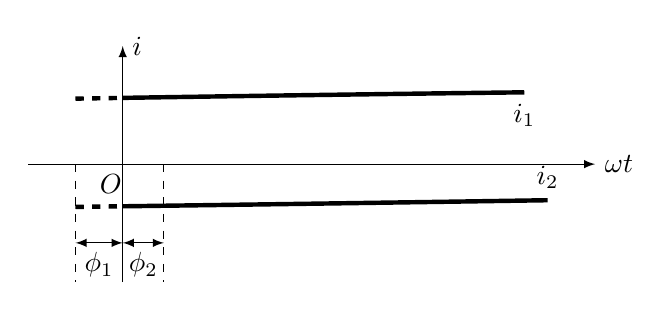
\begin{tikzpicture}[>=latex, xscale=.6]
    \draw [->](-2,0)--(10,0)node[right]{$\omega t$};
    \draw [->](0,-1.5)--(0,1.5)node[right]{$i$};
    \draw [ultra thick] plot[domain=0:9, samples=1000, variable=\x] (\x, {-cos(\x+.7 r)*.7}) node [above]{$i_2$};
    \draw [ultra thick] plot[domain=0:8.5, samples=1000, variable=\x] (\x, {sin(\x+1 r)}) node [below]{$i_1$};
    \draw [ultra thick, dashed] plot[domain=-1:0, samples=100, variable=\x] (\x, {-cos(\x+.7 r)*.7});
    \draw [ultra thick, dashed] plot[domain=-1:0, samples=100, variable=\x] (\x, {sin(\x+1 r)});
    \node at (-.25,-.25){$O$};
    \draw [dashed] (-1,0)--(-1,-1.5);
    \draw [dashed] (3.1416/2-.7,0)--(3.1416/2-.7,-1.5);
    \draw [<->] (0,-1)--node[below]{$\phi_1$}(-1, -1);
    \draw [<->] (0,-1)--node[below]{$\phi_2$}(3.1416/2-.7,-1);
    
    \end{tikzpicture}
